\chapter{Plastic Deformation of Silicon Nanowires}
\label{sec:plastic}

The experiments presented so far were conducted at temperatures high enough to ensure that the irradiated material remains crystalline. This ensures that also the density and shape of the nanowires could be preserved. The following chapter discusses the new effect of plastic deformation, which occurs in the room-temperature ion irradiation of $Si$-nanowires. Some of the experiments were performed together with Stefan Noack and are published in his Master Thesis \cite{noack_sputter_2014} and also in reference \cite{johannes_anomalous_2015}.

\section{Experimental observation of plastic deformation}
\label{sec:expdeformation}

Silicon nanowires where irradiated at room-temperature with high ion fluences of $As^+$ and $In^+$ and/or $Ga^+$ with the goal of forming $Si$-$GaAs$ or $Si$-$InGaAs$ hetero-structures in a further annealing step \cite{prucnal_iii-v_2014,glaser_personal_2015}. To characterize the process, the same individual wires were investigated after each process step, including before and after the ion irradiation. Two exemplary sets of SEM images of these samples can be seen in Figure \ref{deformSEM}. Clearly the nanowires shrank and widened during the ion irradiation, an effect, that has so far not been reported for ion irradiation of $Si$ at such low ion energies. This is a \emph{plastic} deformation caused by the impinging ions, because it is stable even up to high annealing temperatures \cite{prucnal_iii-v_2014,glaser_personal_2015}.

\begin{SCfigure}
	\centering
		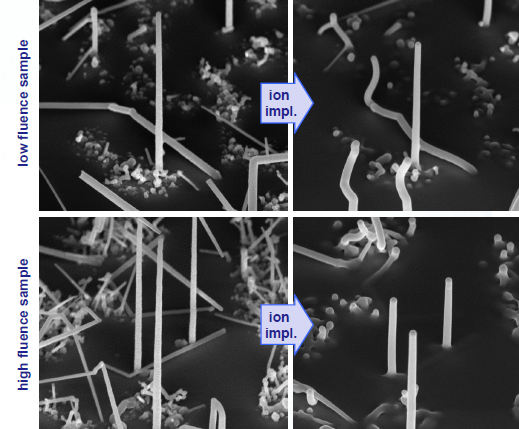
\includegraphics[width=.45\textwidth]{images/deformSEM.png}
	\caption{SEM images of VLS-grown $Si$-nanowires before and after the irradiation with $90\,keV\, In^+$ and $120\,keV\,As^+$ at room temperature, while rotating the sample. The shrinking and widening of the wires is clearly visible and larger in the samples irradiated with the indicated high fluence a), than in those with a comparably low fluence b) of each ion.} 
	\label{deformSEM}
\end{SCfigure}

To investigate this deformation effect systematically, $Si$-nanowire arrays similar to the ones used for the sputtering experiment in Chapter \ref{sec:sisputtering} were irradiated with a set of $Ar^+$ fluences, rotating the samples under the ion beam. Argon ions were chosen for the irradiation to avoid any chemical effects, while the rotation prevented bending of the nanowires, which would have made the quantification of the deformation difficult.  High-resolution SEM images were made after each irradiated ion fluence to observe and quantify the deformation. Using the algorithm described in Chapter \ref{sec:sisputtering}, the profiles for the irradiated nanowires were extracted. In Figure \ref{deformationprofile} the black, red, green and blue lines show the diameter versus height of a single nanowire before and after irradiation with $100\,keV\,\,Ar^+$ up to ion fluences of 1, 3 and $5 \times 10^{16}\,cm^{-2}$ respectively. In this graph, as well as in the inset black profiles, the reduction of the height by $\approx 500\,nm$ and an increase of the diameter, especially at the base, can be clearly seen. 


\begin{figure}[thbp]
	\centering
		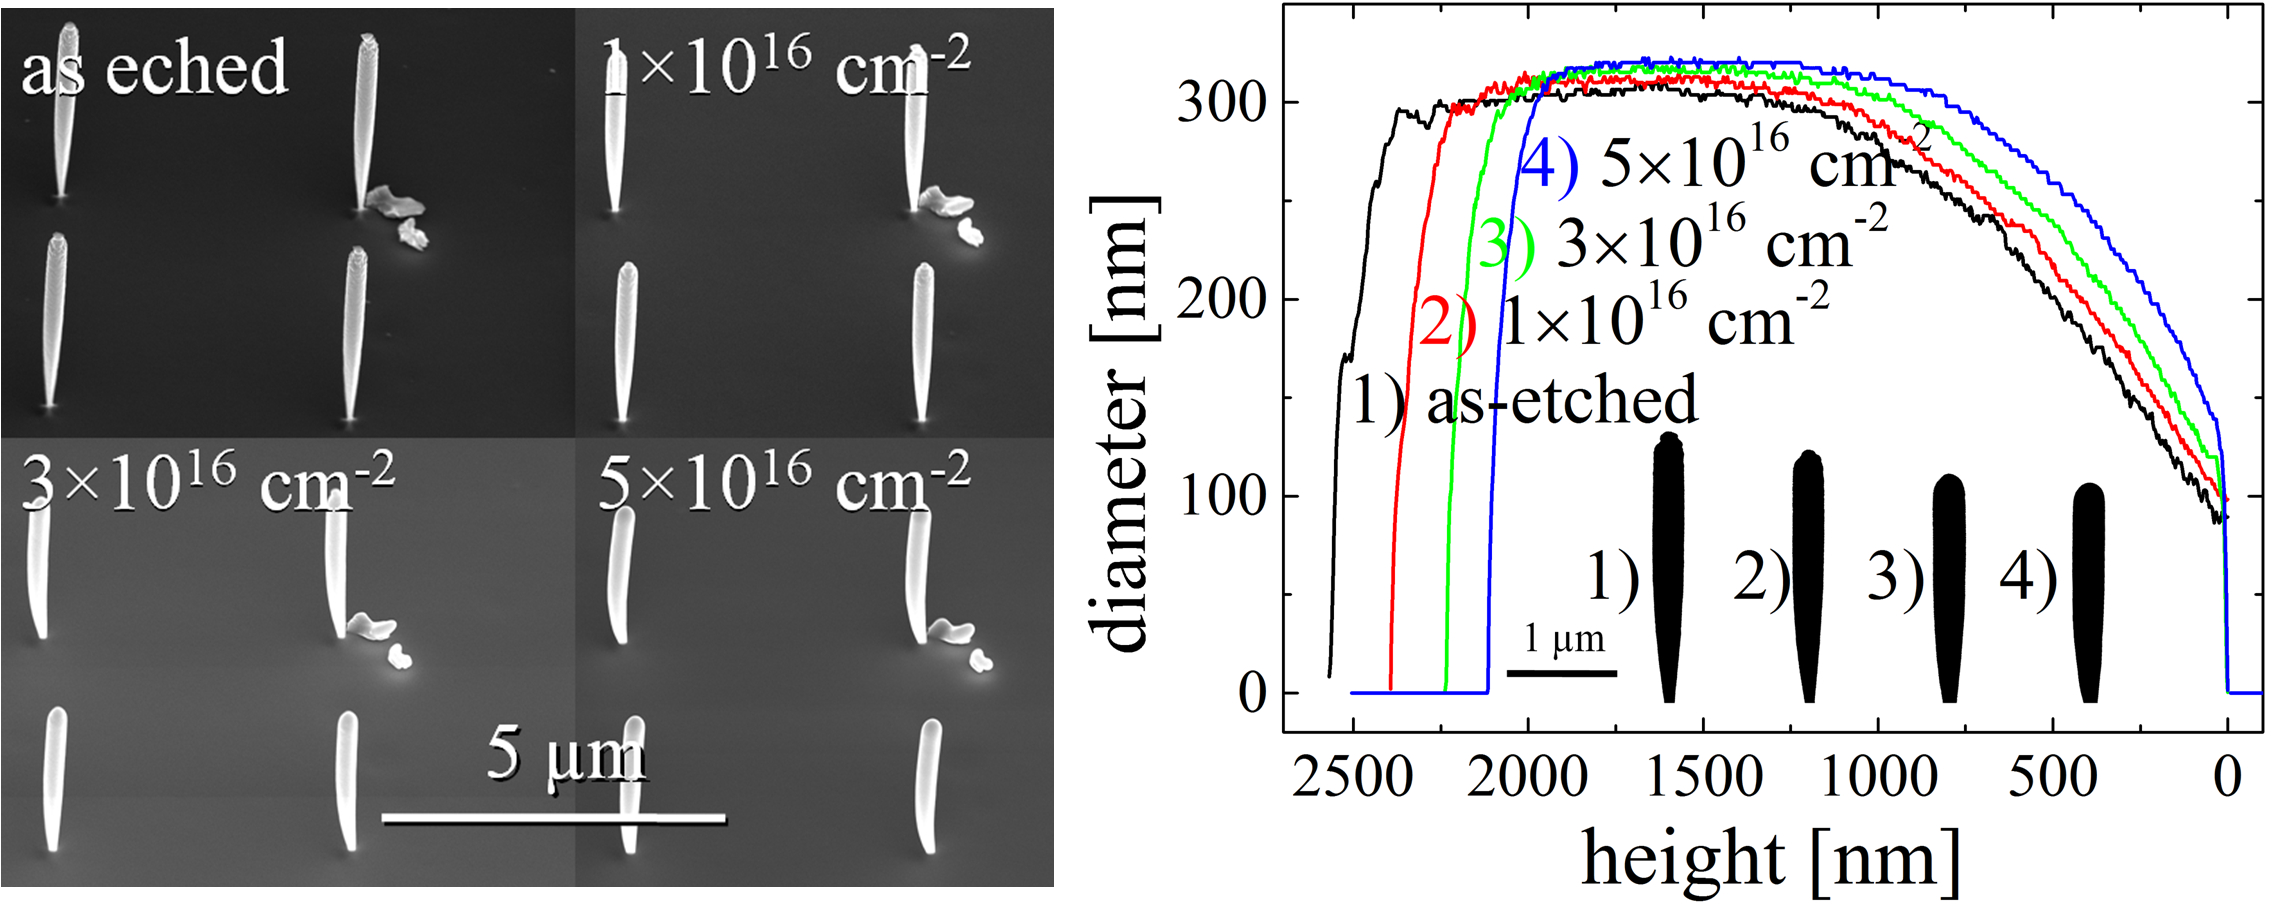
\includegraphics[width=.8\textwidth]{images/deformationprofileandSEM.jpg}
		\caption{Diameter over height of a single $Si$ nanowire irradiated with increasing ion fluences of $100\,keV Ar^+$ ions. The black insets show the profiles of the nanowire after the respective ion fluences extracted from SEM images. In both illustrations the shrinking and widening of the nanowire is clearly visible.} 
	\label{deformationprofile} 
\end{figure}

The plastic deformation does not occur during ion irradiation of cristalline $Si$-nanowires at elevated temperatures, as shown in Chapter \ref{sec:sisputtering}. Only in room-temperature ion irradiation, where the $Si$ amorphization threshold of $10^{14}\,\nicefrac{ions}{cm^2}$ for $100\,keV\,\,Ar^+$ is very low \cite{pelaz_ion-beam-induced_2004}, is the deformation observed. Nanowires first amorphized by ion irradiation and subsequently irradiated at $300^\circ C$ are also deformed. Therefore, it can be concluded, that the plastic deformation under ion irradiation is an attribute of amorphous $Si$. In crystalline $Si$ irradiated at elevated temperatures the efficient recombination of defects or even recrystallization of disordered sections reimposes the long range order of the crystal lattice on the ion-damaged region, preventing any deformation.


\section{Quantification of the Deformation}
\label{sec:quantifydeformation}

The deformation of the nanowires can be roughly quantified by simply fitting a linear trend to the ion fluence dependence of the height of the nanowires. This yields an average of $3\%$ shrinkage per $10^{16}\,\nicefrac{ions}{cm^2}$. Because of outliers with larger deformation the values obtained for the 21 nanowires investigated have a large standard deviation of $3\%$ shrinking per $10^{16}\,\nicefrac{ions}{cm^2}$. The tendency of the nanowires to bend during the ion irradiation made the evaluation of more nanowires impossible. This strong tendency to bend in itself indicates that the deformation process of a single ion impact is not rotationally symmetric across the cross-section of the nanowire. This comes as no surprise as the majority of impacts are off-center and thus clearly unsymmetrical. Also in Figure \ref{deformSEM} the nanowires are clearly only imperfect cylinders as-etched. These starting inhomogeneities and especially the thinned base of the nanowires contributed to their instability during the ion irradiation.

Nevertheless, a more thorough investigation of the deformation is possible in those nanowires which remained upright, by also accounting for the height dependence of the diameter seen in Figure \ref{deformationprofile}. On average a certain number of atoms are displaced by a certain distance along the height $z$ of the nanowire per ion. Considering only the movement along the height $z$, a mass-transport rate (MTR) can be calculated according to equation \ref{MRTequation}:

\begin{equation}  
\begin{split}
    MTR_{(1 \rightarrow 2)} & = [ {}^{1}N\cdot {}^{1}z_{c} -{}^{2}z_{c} \cdot {}^{2}N - ({}^{1}N - {}^{2}N) \cdot {}^{2}z_{c}]/N_{ion} \\
		& = {}^{1}N \cdot ({}^{1}z_{c} - {}^{2}z_{c})/N_{ion} 
	\label{MRTequation}
	\end{split}
\end{equation}

\begin{SCfigure}[50][h]
	\centering
		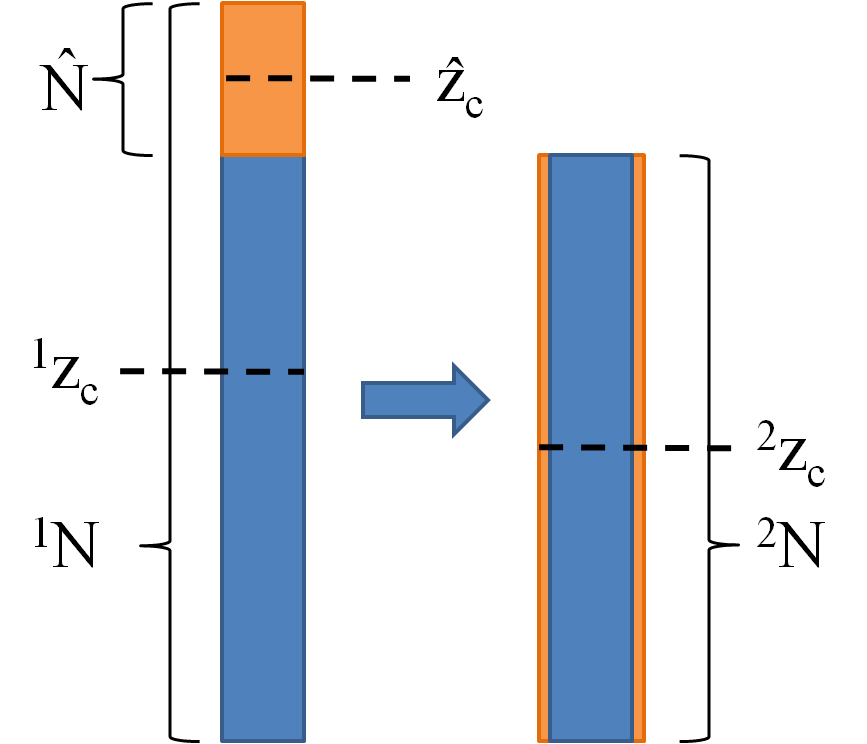
\includegraphics[width=.3\textwidth]{images/MTRillustration.png}
	\caption{Illustration of the mass-transport rate calculation. Displacing ${}^{1}N$ atoms from their average height ${}^{1}z_{c}$ to the average height ${}^{2}z_{c}$ requires the same mass-transport as moving $\hat{N}$ from $\hat{z}_c$ to ${}^{2}z_{c}$, taking into account the number of sputtered atoms ${}^{1}N-{}^{2}N$.}
	\label{MTRillustration}
\end{SCfigure}

In equation \ref{MRTequation} and Figure \ref{MTRillustration}, ${}^{1/2}z_{c}$ is the height of the center of mass of the nanowire with the top left index indicating before ($^1$) and after ($^2$) ion irradiation respectively. The number of atoms at height $z_i$ can be calculated from the local radius $r_i$. Summing up the height weighted by the number of atoms at that height $z_{c} \cdot N = \sum_i{\pi r_i^2 h \cdot \rho \cdot z_i}$ and dividing this by the total number of atoms $N = \sum_i{\pi r_i^2 h \cdot \rho}$ in the nanowire gives us $z_{c}$. The sums are over all slices $i$ of height $h = 1\,pixel = 2.7\,nm$ (typically) each. The number of ions that hit the nanowire during the irradiation of ion fluence $\Phi_{12}$ between making SEM images $1$ and $2$ is $N_{ion} = \sum_i{({}^{1}r_i+{}^{2}r_i)}$ $\cdot sin(45^\circ) \cdot h \cdot \Phi_{12}$. The last term in equation \ref{MRTequation} accounts for the influence of sputtered atoms. Just as in Chapter \ref{sec:sputter} on sputtering, the sputter yield could be calculated by $({}^{1}N - {}^{2}N)/N_{ion}$. Figure \ref{MTRillustration} illustrates two interpretations of the MTR calculation. Because only the displacement along $z$ is considered, the direct interpretation of equation \ref{MRTequation} of moving ${}^{1}N$ atoms from their center of mass ${}^{1}z_{c}$ to a new center of mass ${}^{2}z_{c}$ is equivalent to moving the atoms which are `missing' at the top of the nanowire after the irradiation ($\hat{N}$, orange volume in Figure \ref{MTRillustration}) from their center of mass $\hat{z}$ to ${}^{2}z_{c}$, and subtracting the sputtered atoms. This evaluation yields an average mass-transport rate of $1.2\cdot10^4 \,\nicefrac{atoms \cdot nm}{ion}$ with a standard deviation of $7\cdot 10^3\,\nicefrac{atoms \cdot nm}{ion}$. Again the large standard deviation is mainly caused by outliers with larger deformation, as can be seen in the histogram of the evaluated mass-trasport rates for a couple of nanowires in Figure \cite{MTReval}.

\begin{SCfigure}[50][h]
	\centering
		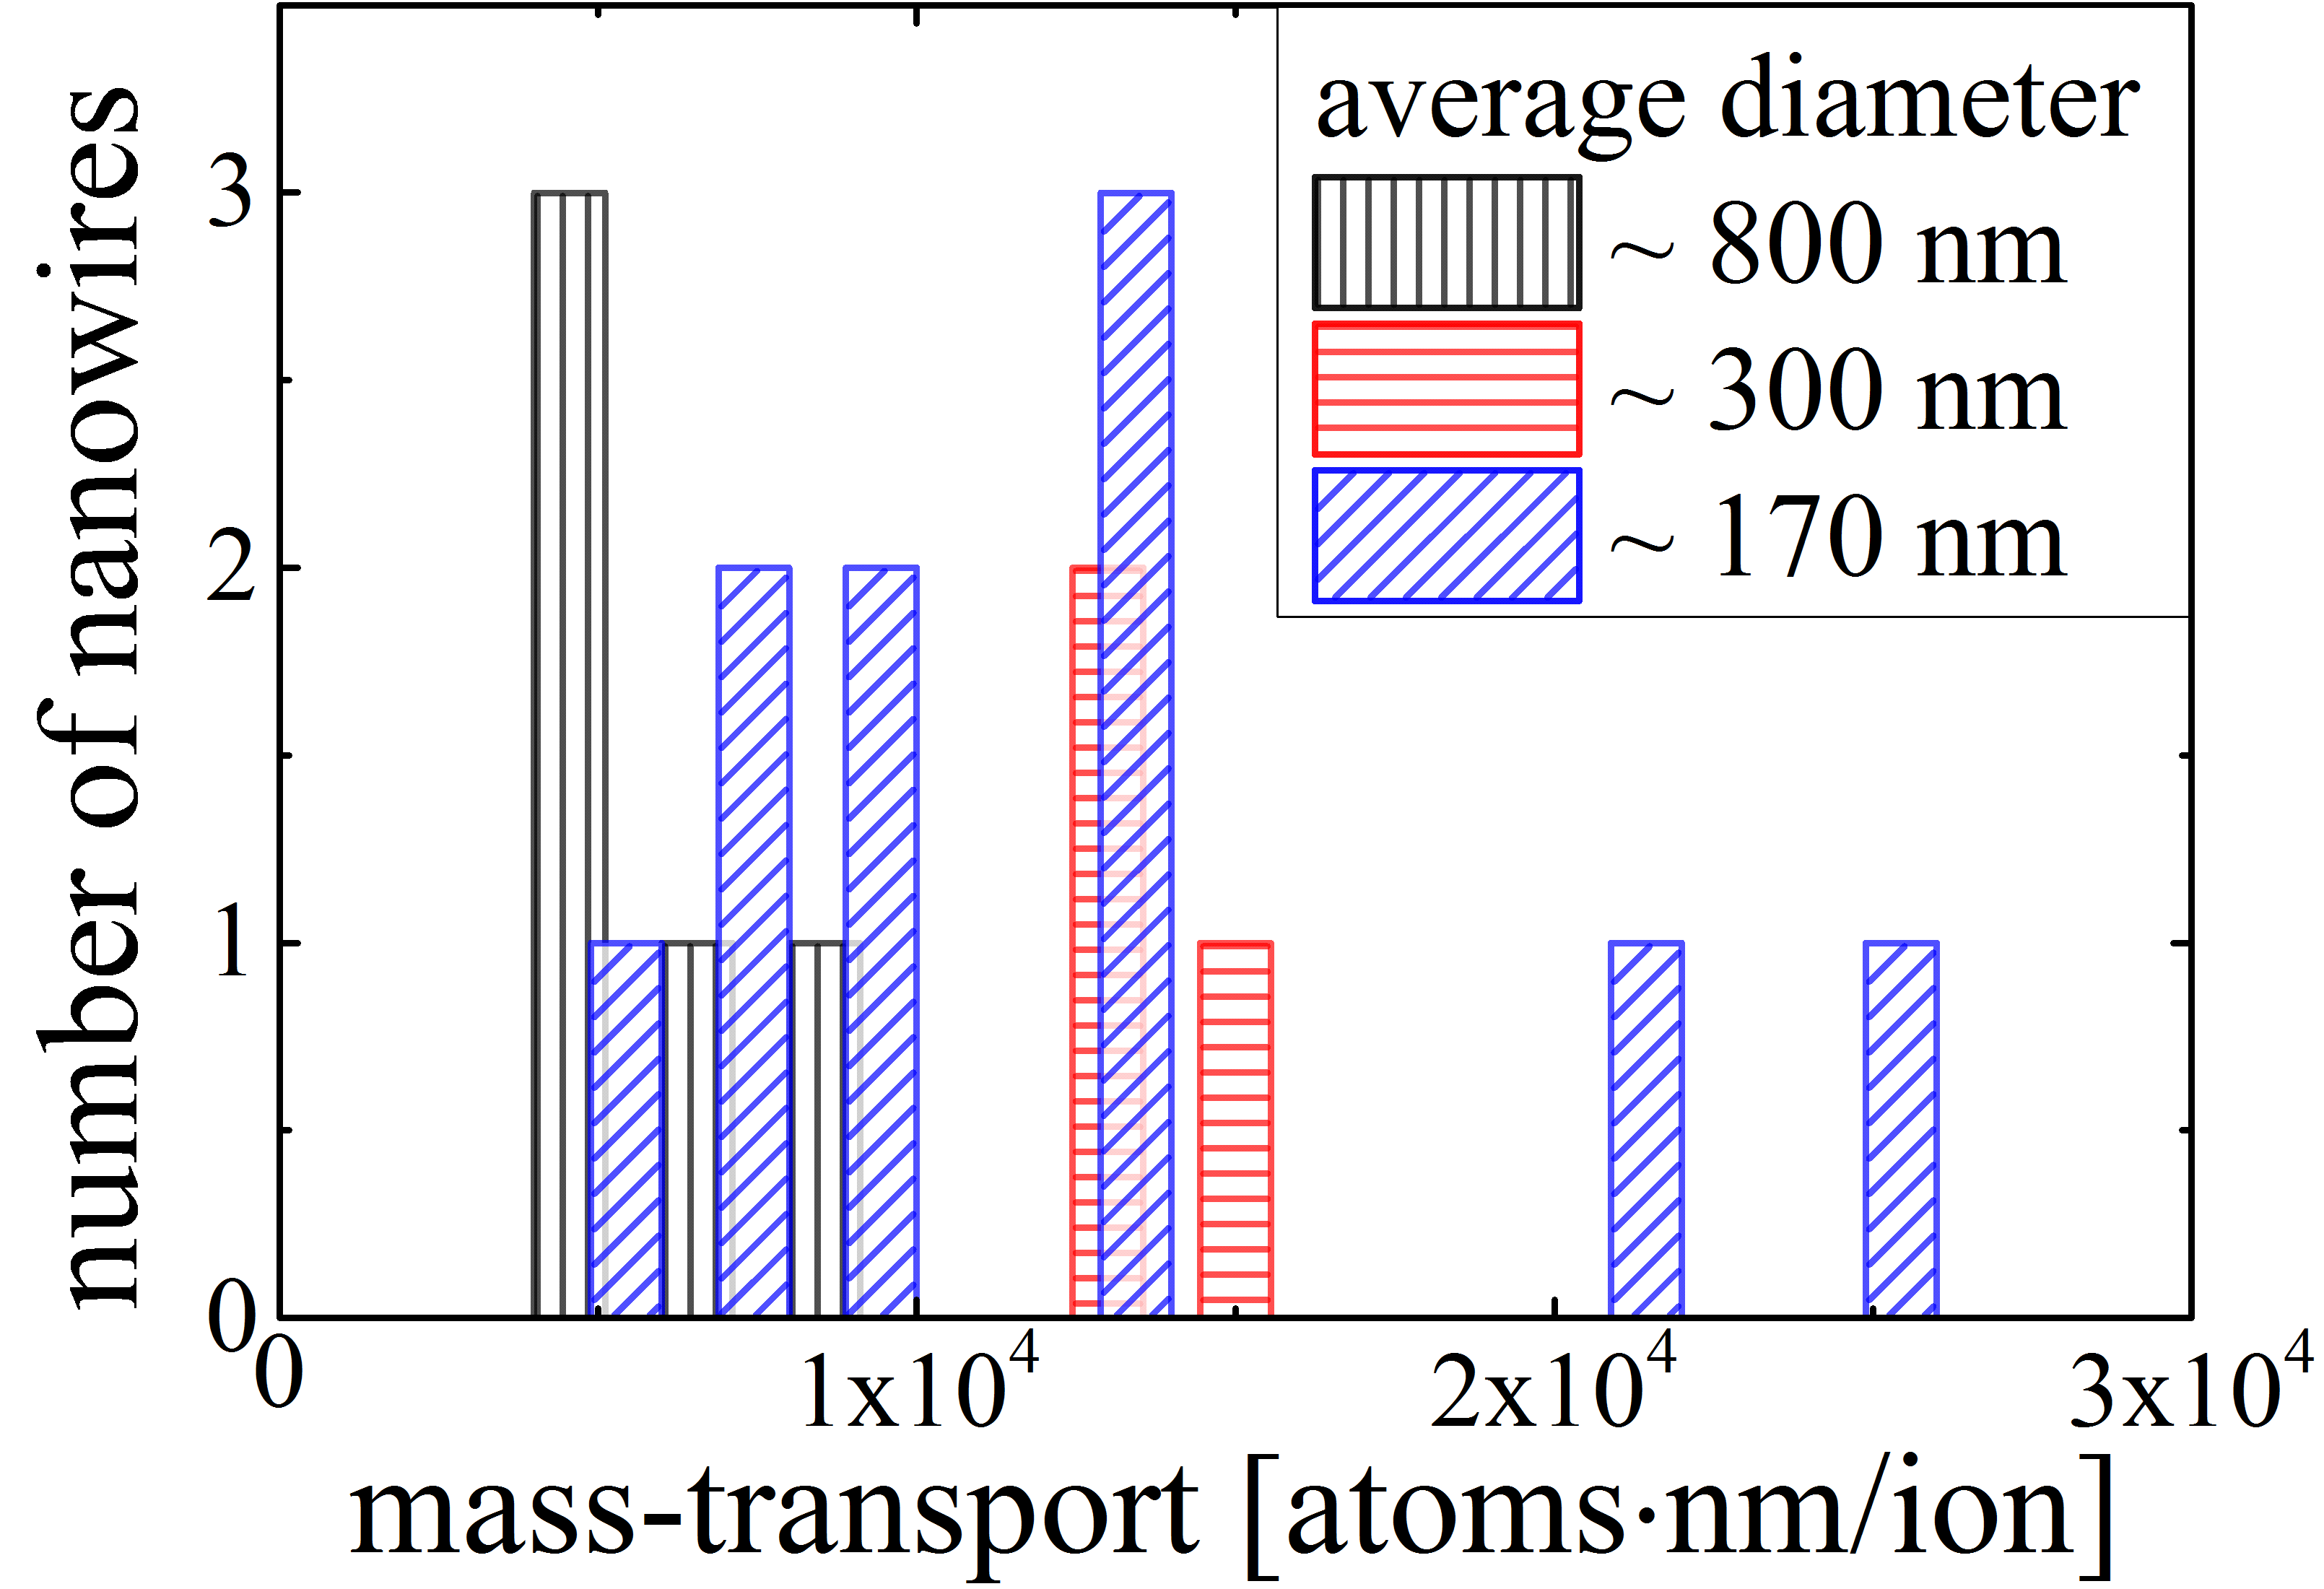
\includegraphics[width=.5\textwidth]{images/MTReval.png}
	\caption{Histogram of the results of all mass-transport rates evaluated from the deformation of individual nanowires. Because of the large spread of the data points, no significant correlation between the average diameter nor the ion energy can be shown.}
	\label{MTReval}
\end{SCfigure}


\section{Knock-on transport of mass}

A possible explanation for this observed plastic deformation can be sought in the linear cascade theory, which is applicable for the cascades of $100\,keV\,\,Ar^+$ in $Si$: In a collision cascade following an energetic ion impinging a solid, atoms will be preferentially `knocked-on' along the propagation direction of the impinging ion. This causes an inhomogeneous distribution of interstitials and vacancies and effectively, mass is transported `downstream' along the ion beam. In an amorphous material it is not clear what constitutes an `interstitial' or a `vacancy', but a local excess of vacancies can be understood as a locally decreased density, while an interstitial excess corresponds to an increased density. A local density gradient is not stable, because the density of amorphous $Si$ before and after ion irradiation is not significantly different \cite{pelaz_ion-beam-induced_2004}. Therefore, the density gradient introduces stress in the material, which can relax by plastic deformation, possibly enabled by a decreased viscosity caused by further ion irradiation \cite{snoeks_stress_1997,hu_burrowing_2002,mayr_mechanisms_2003,mayr_effect_2003}. 

As was shown in Chapter \ref{sec:sputter} on sputtering, BCA simulation software can accurately reproduce linear collision cascades. Therefore, a comparison between the experiments and a simulation with \emph{iradina} can evaluate whether the deformation observed in the experiment can be accounted for by knock-on mass transport. Figure \ref{deformationBCA}a shows the $600\,nm$ long $Si$ cylinder with a diameter of $200\,nm$ implemented in \emph{iradina} with $2\times2\times2\,nm^3$ voxels in a simulation volume of $204\times204\times600\,nm^3$. The $100\,keV\,\,Ar^+$ ions impinge at an angle of $45^\circ$ to the $z$-axis. They strike the cylinder distributed uniformly along the $y$-direction at height $z=0$. Figure \ref{deformationBCA}d shows the resulting distribution of interstitials on the cross-sectional slice through the middle of the nanowire along the $xz$ plane. This can be seen as an approximation for the distribution of the nuclear energy loss and shows the mean extent of the collision cascade. Figure \ref{deformationBCA}e shows the same cross-section after subtracting the number of vacancies produced per ion from the number of interstitials. The excess of vacancies along the impinging plane (blue cone in the cross section) enveloped by two red planes of excess interstitials shows that there is a high probability for the ions to hit a target atom with a large impact parameter. This changes the ions path only little and displaces the target atom in an direction perpendicular to the ion beam. Superimposing many collisions along the $y$ direction leads to the formation of one vacancy rich and two interstitial rich planes. The $xy$-plane in \ref{deformationBCA}b shows the sum over the height $z$ of the difference between interstitials and vacancies plotted to the same color scale. The illustration is dominated by vacancies at the surface of the cylinder, which are left behind by sputtered atoms. 

The height distribution (summing over the radial $xy$ plane) of the interstitials, vacancies and leaving atoms is shown in \ref{deformationBCA}c. As expected, the majority of sputtered atoms originate near the impact height. The lines showing the interstitials and vacancies overlap in this illustration. The vacancies subtracted from the sum of interstitials and leaving atoms is plotted along the height in \ref{deformationBCA}f. Because a displaced atom, leaving behind a vacancy, is either sputtered or becomes an interstitial, the sum over all heights of of this graph is zero. The strong oscillation around $z=0$ in \ref{deformationBCA}f is caused by the previously discussed displacement of target atoms at an angle almost perpendicular to the ion beam for large impact parameters. This oscillation is very sensitive to the voxel-size, because, in effect, the voxel size defines a recombination length, and interstitial and vacancy rich regions are mixed in larger voxels. On the other hand, the excess of vacancies near the impact point ($\le 70\,nm$) and of interstitials further down along the ion's path ($\approx 100\,nm$) is not sensitive to the voxel size. It can be used to quantify the knock-on mass transport by multiplying the plotted values by their height and integrating over all heights. The influence of the short range oscillation immediately around the impact point disappears, because here $z \approx 0$ is small. The value obtained from this calculation is $78\pm1\,\nicefrac{atoms \cdot nm}{ion}$. Clearly this value is to low to account for the large deformation observed in the experiment where a mass-transport rate of $\ge 1\times 10^{4}\,\nicefrac{atoms \cdot nm}{ion}$ was assessed.

\begin{Figure}[h]
	\centering
		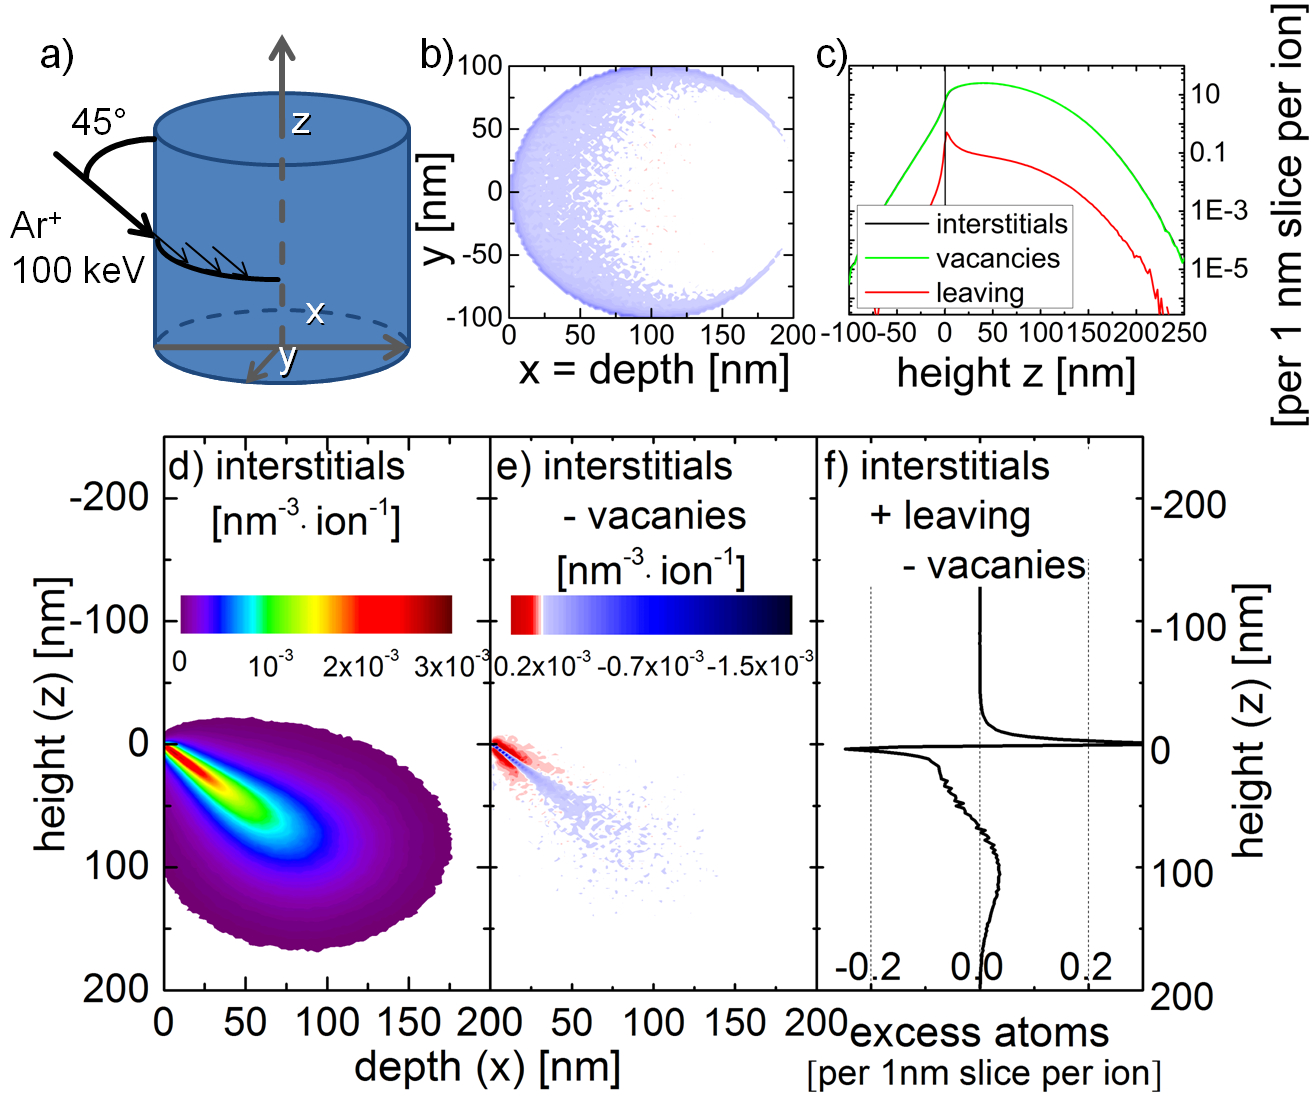
\includegraphics[width=.9\textwidth]{images/deformationBCA.jpg}
		\caption{a) Illustration of the simulated irradiation geometry. All $Ar^+$ ions of $100\,keV$ energy hit the nanowire volume at the same height and at an angle of $45^\circ$ with respect to the nanowire axis $z$. The created interstitials in the radial cross-section through the middle of the simulated nanowire is shown in d). This distribution is effectively an illustration of the nuclear energy loss. In e) the vacancies are subtracted from the interstitials for the same cross-section. Summing this difference over all heights gives the radial distribution shown in b). The clear dominance of vacancies near the surface is caused by sputtering. The axial profile of the interstitials, vacancies and leaving (sputtered) atoms plotted in c) over the height relative to the impact plane shows that most atoms are sputtered at the impact height. Note that the plots of vacancies and interstitials overlap. The vacancies subtracted from the sum of interstitials and sputtered atoms plotted over the height in f) shows mass transport along the ion's path. Apart from the strong oscillation at the impact height, there is a deficiency of atoms close to the impact height ($\le 70\,nm$) and an excess centered around $100\,nm$ down from the impact height.} 
	\label{deformationBCA}	
\end{figure}

For all simulations a reasonable value for crystalline $Si$, $15\,eV$ \cite{corbett_production_1965}, was used for the displacement energy, which governs the creation of interstitials and vacancies in the simulation, as discussed in Chapter \ref{sec:simion}. However, in amorphous materials it is questionable what this value is supposed to mean, because point defects are not well defined. Therefore, simulations where repeated with the displacement energy set to $0\,eV$. As expected, the number of `vacancies' and `interstitials' now produced by the simulation increased dramatically. However, the long range difference between `vacancies' and `interstitials' seen in Figure \ref{deformationBCA}f remains unchanged. This is an indication that the knock-on mass transport is dominated by the rare events where ions hit the target atoms directly, with low impact parameters. In these cases, a large amount of energy is transferred to the displaced atom leading to a long trajectory, preferentially in line with the ion's momentum. On the other hand, atoms displaced with lower energies are much more numerous, but travel much shorter distances and in a randomly orientated direction. This is because most of the low energy displaced atoms are generated at the end of a branch of the collision cascade, the orientation of the branch having previously been randomized by higher energy collisions. The other low energy recoils originate from collisions with a high impact parameter, which leads to a large angle between the incoming particle's and the displaced particle's momentum, as seen near the impact point as a separation of interstitials and vacancies in Figure \ref{deformationBCA}e and as the short range oscillation in Figure \ref{deformationBCA}f. These large angle recoils do not contribute significantly to long range mass transport.

\clearpage
\section{Ion irradiation at large angles of incidence}

If knock-on mass-transport is not the main contribution to the deformation, the question arises whether the direction of the plastic deformation in the nanowires is related to direction of the ion beam. Will an ion irradiation from `below the substrate' towards an unconstrained end of the nanowire also shrink the nanowire, or stretch it out? 

Nanowires attached to a substrate are obviously not suited to answering this question, so a method to irradiate nanowires while rotating them at angles greater than $90^\circ$ to the ion beam was devised. This was achieved by attaching a $Si$ nanowire grown epitaxially on a $Si$ wafer to an $Au$ microwire, which can suspend the nanowire at arbitrary angles in the irradiation chamber. The process is shown in Figure \ref{reverseFIB}. Platinum deposition by e-beam was used to ``glue'' the nanowire to the micro-manipulator in the FIB, after which the nanowire was cut from the substrate with the $Ga$-FIB. Using the $Pt$-deposition and $Ga$-FIB again, the nanowire was subsequently attached to the tip of a sharpened $Au$-microwire, which was previously glued to a piece of wafer for handling and also placed in the FIB chamber. The VLS-grown $Si$ nanowires, similar to those shown in Figure \ref{deformSEM}, were used for this experiment, because they were readily available in longer lengths ($>10\mu m$) than the etched nanowires.

\begin{Figure}[thbp]
	\centering
		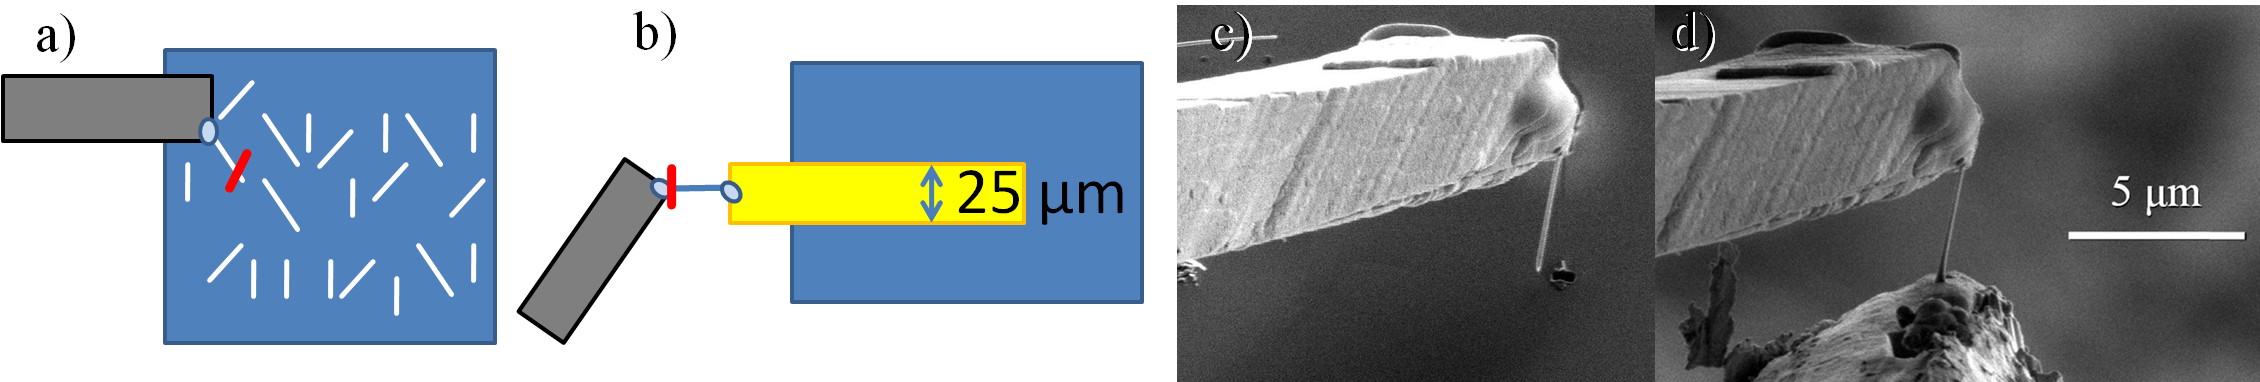
\includegraphics[width=0.99\textwidth]{images/reverseFIB.jpg}
	\caption{Illustration of the nanowire-on-microwire fabrication in a FIB system. The schematic a) and SEM image c) show the nanowire first glued to the micro-manipulator in the FIB by $Pt$-deposition (light blue ellipse), then cut from the substrate with the $Ga$-FIB (red line). Images b) and d) Illustrate the subsequent gluing to an $Au$ microwire with $Pt$-deposition and the final cut with the $Ga$-FIB to release the nanowire from the micro-manipulator.}
	\label{reverseFIB}
\end{Figure}

The nanowire-on-microwire samples consisted of typically $3-5$ nanowires, each attached to an $Au$-microwire and arranged in the irradiation chamber on a rotatable stage at an angle of $135^\circ$ to the ion beam, as shown schematically in Figure \ref{reverseangle}a. The alignment of the nanowires to their microwire support was found to be crucial, because any shadowing of a nanowire from the ion beam an one side would lead to extreme bending of the nanowire. Only a single nanowire was found straight enough to evaluate quantitatively for more than one ion fluence irradiation step. The SEM images of this nanowire are shown in Figure \ref{reverseangle}b-f from a perspective perpendicular to the axis of rotation and rotated by the indicated angle around this axis. The left SEM images show the unirradiated nanowire, while the center and right images were made after the irradiation of $1\times10^{16}\,cm^{-2}$ and $3\times10^{16}\,cm^{-2}$ $100\,keV\,\,Ar^+$, respectively. The unirradiated nanowire is straight and $3.9\,\mu m$ long. The irradiated nanowire shows some bending, so the length had to be determined from a perspective were the curvature of the nanowire is in plane with the image. A fifth order polynomial was fitted to the bent shape and the length of the nanowire was thus determined to be $3.5\,\mu m$ after $1\times10^{16}\,cm^{-2}$ (\ref{reverseangle}b) and $3.2\,\mu m$ after $3\times10^{16}\,cm^{-2}$ (\ref{reverseangle}f). The nanowire shrank with a similar deformation rate to the previously reported $3\%$ strain per $10^{16}\,\nicefrac{ions}{cm^2}$, even though the irradiation was directed towards its free end!

\begin{Figure}[thbp]
	\centering
		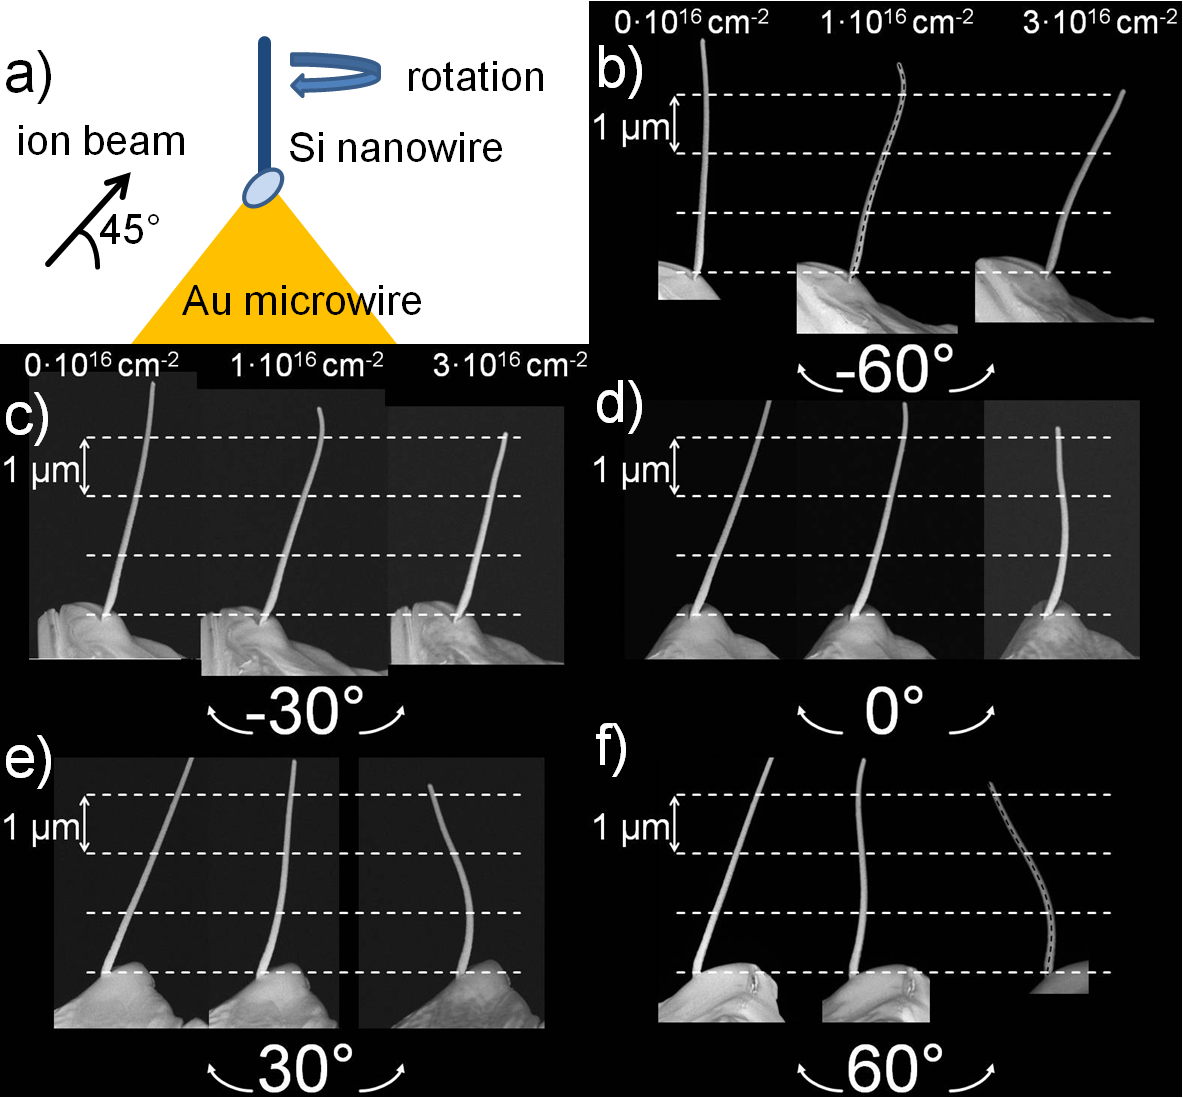
\includegraphics[width=8cm]{images/reverseangle.jpg}
	\caption{ a) Illustration of the nanowire-on-microwire irradiation setup. b) - f) SEM images of the same nanowire as-mounted (left SEM images), after irradiation with $1\times10^{16}\,cm^{-2}$  (center images), and $3\times10^{16}\,cm^{-2}$ (right images) $\,100\,keV Ar^+$ ions. The SEM images where taken with the nanowire rotated by the indicated angle from a perspective perpendicular to the angle of rotation. The length of the nanowire after irradiation is determined in b) and f) along the dashed lines.}
	\label{reverseangle}
\end{Figure}

\section{The proposed deformation mechanism}

This experiment shows with certainty that the knock-on mass-transport is not the main contributor to the observed deformation, because it would have to be directed along the ion beam. The discussion of a possible model for the deformation will be easier by addressing similar effects and the way that simulation tools were used to understand them. The BCA MC simulation tools available inherently neglect all collective movement of atoms within the target. A field of study that has already faced the limitation of neglecting the local temperature in ion irradiation, is the irradiation with swift, heavy ions. At energies well beyond $MeV$, the assumption that the dominating effects will be described by binary collisions between the ion and target atoms is false. At high energies and ion masses a significant amount of energy will be transferred form the ion to the electronic system of the target. Through the relaxation mechanisms of the electronic system a part of this energy will be converted to heat in the lattice. Under certain conditions this will form ``ion-tracks'' in the target. One approach to understand the formation and behavior of ion-tracks is to simulate the longitudinal distribution of the deposited ion energy in the target with BCA tools (typically SRIM) and to evaluate the local temperature in a second step by following the deposited energy according to thermodynamic considerations. A good review of such ``thermal spikes'' can be found in in reference \cite{wesch_effect_2004}. 

Such a thermal spike approach was successful for the description of the plastic deformation by swift heavy ion irradiation according to Trinkaus and Ryazanov \cite{trinkaus_viscoelastic_1995} and in the understanding of material properties governing the direction of the deformation \cite{hedler_amorphous_2004,hedler_boundary_2005}. When nanoparticles are deformed \cite{snoeks_colloidal_2000,snoeks_colloidal_2001,van_dillen_anisotropic_2001,dillen_energy-dependent_2001,dillen_ion_2003,dillen_ion_2004} an adapted version of the model by Trinkaus can be applied and the effect dubbed ``ion hammering'' \cite{klaumunzer_ion_2004}. In short, according to this model the local temperature leads to a transient `liquid' phase in the cylindrical volume of material around the ion's path. Within the cylindrical geometry, the deformation by thermal expansion is anisotropic and because stresses can relax in the low-viscous volume, this is plastic deformation. As with the deformation shown in the present work, the deformation is not observed in materials that remain crystalline during the swift-heavy ion irradiation, because the long range order of the crystal lattice is reinforced upon the recrystallization during cooling. The problem with directly applying this model to the given situation is that the total energy density in the collision cascade of $100\,keV\,Ar^+$ in $Si$ is a low $\frac{dE}{dx} = 36\,\nicefrac{eV}{nm}$, of which the electronic energy loss is roughly half. Also, the lowest ion energy for which plastic deformation of silica nanoparticles is reported is $300\,keV Xe^+$ \cite{dillen_ion_2003}. Here, the energy loss is merely $\frac{dE}{dx} = 120\,\nicefrac{eV}{nm}$ with $20\,\%$ lost to the electronic system. The threshold for ion tracks, however, is given at $\frac{dE}{dx} \geq 1\,\nicefrac{keV}{nm}$ by Trinkaus et al. \cite{trinkaus_viscoelastic_1995}.

The alternative to thermodynamic considerations after a MC BCA simulation are full MD simulations, where the trajectory and interaction of every atom or ion in the simulation volume is followed. This naturally includes all thermal effects, but is limited by computing power to a low number of atoms and thus a severely limited volume of material. Investigations of the self-irradiation of $10\,keV\,Si$ and various metals \cite{nordlund_defect_1998} revealed the formation of nanoscale `liquid' pockets. The term `liquid' must be used with care, because it refers to a thermodynamical state of matter while the simulation timescale does not allow the assumption of thermodynamic equilibrium. Nevertheless, a sufficiently large number of atoms gain much kinetic energy (say `are hot') to make the assumption effects such as a reduced viscosity and thermal expansion safe. The interesting point of this example is that the energy in the collision cascade was quite low, so that the trajectory of the initiating particle could also have been accurately simulated according to the BCA. A more recent MD investigation by Baumer et al. gets even a step closer to the presented experimental results, in that it predicts plastic deformation in metallic glasses irradiated with high energy neutrons \cite{baumer_prediction_2014}. The collision cascades are initiated in $a$-$Cu_{50}Nb_{50}$ by assuming primary knock-on atoms of $475\,keV Nb$. This atomistic study explicitly shows that plastic deformation caused by thermal expansion and stress relaxation can be anisotropic also in collision cascades which do not have the high energy density and symmetry required by the Trinkaus model \cite{trinkaus_viscoelastic_1995}. Somewhat contrary results were obtained by Mayr et al. \cite{mayr_mechanisms_2003} where $10\,eV$ to $100\,keV$ recoils of $Cu$ and $Ti$ in $a$-$CuTi$ were simulated. That study comes to the conclusion that the viscous flow is dominated by ion induced point defects. It does not propose that knock-on atoms initiate the deformation, but rather, that thermal effects do not provide the main contribution to the reduced viscosity observed during ion irradiation.


\begin{Figure}[thbp]
	\centering
		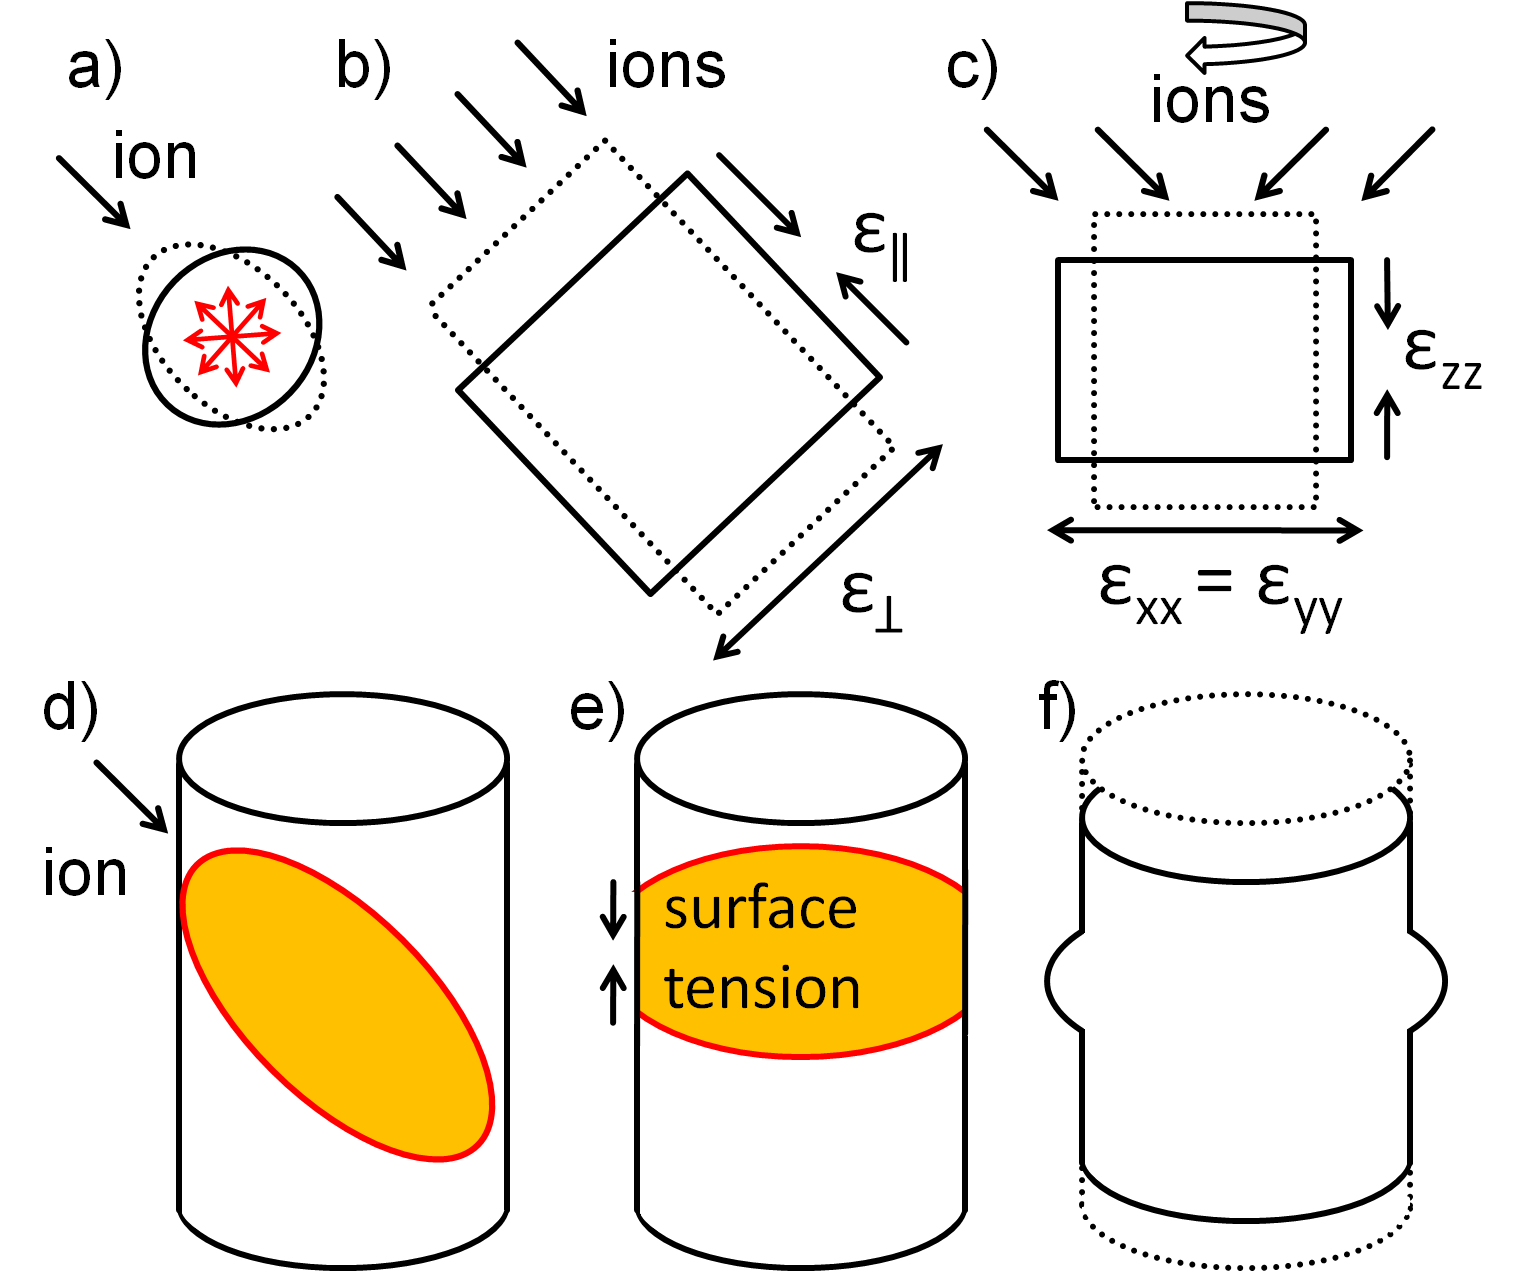
\includegraphics[width=8cm]{images/deformationmodel.jpg}
	\caption{a) - c) Illustration of a deformation model analogous to ion hammering. a) The collision cascade from a single impinging ion heats an approximately ellipsoidal volume of the target material. The internal pressure will lead to an expansion towards a more spherical shape, which is retained upon cooling. b) The net effect of many ions is thus a contraction parallel to and an expansion perpendicular to the ion beam. For no change in density $\epsilon_\parallel = -2\epsilon_\perp$ has to hold. c) Under rotational symmetry this deformation translates to a contraction in the rotational axis $z$ and an expansion in the perpendicular $x-y$ plane with $\epsilon_{zz} = -2\epsilon_{xx} = -\epsilon_\perp$. In d) - f) the alternative, surface tension driven deformation is illustrated. The collision-heated volume of target material shown in d). A significant slice of the nanowire shown in e) thus has a reduced viscosity. The surface energy is reduced by an increase in the local diameter of the nanowire, leading to a shortened and thickened nanowire segment shown in f).} 
	\label{deformationmodel}
\end{Figure}

The effect of anisotropic deformation within the collision cascade induced by the ion irradiation of nanowires is shown in Figure \ref{deformationmodel}a - c. An approximately ellipsoidal volume of the target material is heated by the collision cascade. It expands, becoming more spherical and the anisotropic deformation is retained after cooling. The superimposition of many collision cascades with a similar effect leads to a net contraction along the ion beam $\epsilon_{\parallel} < 0$ and an expansion perpendicular to it $\epsilon_{\perp} > 0$, as shown in \ref{deformationmodel}b. To maintain constant density $-2\cdot\epsilon_{\perp} =  \epsilon_{\parallel}$. The rotational average of this deformation around the $z$-axis, as illustrated in \ref{deformationmodel}c, works out to be a contraction along the $z$-axis $\epsilon_{zz} = \nicefrac{1}{2} \epsilon_{\parallel}$ and a corresponding expansion in the $xy$-plane for an angle of $\pm\, 45^\circ$ between the ion beam and the $z$-axis. The $z$-axis represents the nanowire axis, while the $xy$-plane is parallel to the nanowire diameter. Thus, the deformation rate of $d\epsilon_{zz}/d\Phi = 3\%$ strain per $10^{16}\,\nicefrac{ions}{cm^2}$ extracted from a linear fit to the reduction of the nanowire height can be transformed into a strain rate parallel to the ion beam of $d\epsilon_{\parallel}/d\Phi = 6\%$ strain per $10^{16}\,\nicefrac{ions}{cm^2}$, or $6\cdot 10^{-18}\,\nicefrac{cm^2}{ion}$. This is much less than the values for the studies at higher energies reported in literature. In reference \cite{dillen_ion_2003} a strain rate of $10^{-16}\,\nicefrac{cm^2}{ion}$ were reported for $300\,keV\,Xe$ in silica nanoparticles and ref. \cite{baumer_prediction_2014} even arrives at $10^{-15}\,\nicefrac{cm^2}{ion}$ with MD calculations in bulk. 

The quantitative discrepancy between the deformation observed in the experiments presented here and published studies may be attributed to the lower ion energy and one may gain confidence in this model because of the qualitative similarity to the MD simulations by Baumer et al. \cite{baumer_prediction_2014}, which also show a deformation anisotropy at relatively low ion energies. However, a further, major difference between the MD simulation and the experiments presented here is the fact that in the presented experiments the collision cascade is not in bulk, but in a nanostructure were there is not much material around and it is not distributed around the cascade isotropically. If the ellipsoidal volume intersects the nanowire surface, the pressure from the thermal expansion can vent outward removing the force needed to drive the deformation.

A favorable model relies on the surface tension as a driving force of the observed plastic deformation. In Figure \ref{deformationmodel}d the relation between the nanowire and collision cascade is shown. Because there is not much material around, the temperature in a sizable volume of the nanowire will remains elevated for some time \cite{borschel_ion-solid_2012,greaves_enhanced_2013,anders_sputtering_2015,johannes_ion_2015}. In addition, the ion irradiation itself reduces the viscosity locally \cite{snoeks_stress_1997,hu_burrowing_2002,mayr_mechanisms_2003}, allowing the surface tension to deform the nanowire by increasing the radius locally. The local increase in diameter reduces the total surface area and thus the surface energy. The nanowire subsequently becomes shorter and wider, as shown in Figure \ref{deformationmodel}f. Further evidence for the surface tension driven plastic deformation can be found in the SEM images in figures \ref{deformSEM} and \ref{deformationprofile}a. The nanowires look smooth and `molten' after the ion irradiation, which may be an indication that they underwent a temporary, local transition into a phase of low viscosity. This smoothing is not necessarily observed in ion-irradiated nanowires, as the $Si$-nanowires irradiated at elevated temperatures, shown in Chapter \ref{sec:sisputtering}, Figure \ref{sputtering_exp}, do not show such a rounded top facet.

If the plastic deformation is surface tension driven, it should show a strong diameter dependency, as both the surface tension itself, as well as the average ion-deposited local energy density and with it the viscosity are diameter dependent. The first model based on an anisotropic deformation within a collision cascade is only diameter dependent because a limited volume of material is  deformed. If the nanowires' diameter increases, the total volume increases and thus the deformation reduces proportionally. The extremely large nanowires on the samples investigated in this thesis indeed barely show any deformation, however, this is expected for both models and thus can not be used to distinguish between the two. As stated earlier on, it was unfortunately not possible to investigate enough deformed nanowires to come up with a useful diameter dependency of the deformation.

Nevertheless, there is no inherent reason why the process of anisotropic deformation within a collision cascade should not be observable in bulk samples, yet there are no studies published on straining amorphous bulk silicon at these low ion energies. The bending of thinned $Si$-wafers would be measurable in experiments similar to those in references \cite{volkert_stress_1991,massl_stress_2008}. The straining rate of $6\%$ strain per $10^{16}\,\nicefrac{ions}{cm^2}$ in a layer of $\approx 300\,nm$, which can be predicted with from the results presented in this thesis, produces sufficient bending for said experimental method \cite{flinn_measurement_1987}. It is unfortunately not clear, whether the lack of a publication of bulk deformation at low ion energies is due to the absence of the effect in bulk, or merely the absence of an experimental investigation of it. While the large interest in $Si$ and ion irradiated $Si$ in particular makes the latter seem somewhat unlikely, it can not be excluded.

Apart from the bulk and diameter-dependent deformation experiment already suggested, a further experiment, which could distinguish which of the two models applies, is the ion irradiation of the nanowires radially, at $90^\circ$ between the nanowire axis and the ion beam. In this irradiation geometry, if the first model similar to ion hammering applies, the irradiation should produce slowly elongating wires with a reduced radius, because the positive strain $\epsilon_{\perp}$ is now parallel to the nanowire axis. On the other hand, if the surface tension driven model is applicable the nanowires will shrink regardless of the ion irradiation angle. Naturally, a similar nanowire-on-microwire setup to the one for irradiation at $135^\circ$ could be used to irradiate at $90^\circ$. This experiment was undertaken, but, unfortunately, it turns out that ion irradiation at $90^\circ$ is extremely prone to bending the nanowires. The bending is attributed to the $Pt$ deposited used to attach the $Si$ nanowire onto the $Au$ microwire in the FIB. This deposition is concentrated at the base and on one side of the nanowire and thus suppresses the rotational symmetry of the deformation, leading to bending. In the irradiation at $135^\circ$ the base of the nanowire, where the $Pt$ is deposited, is shadowed from the ion beam by the microwire so that the nanowires are less likely to bend in this configuration. Due to the bending, the angle between the nanowire and the ion beam varied during a rotation cycle, so that a conclusive discrimination between the models can unfortunately not be made. 

In conclusion, the surface tension is the most likely driving force for the observed plastic deformation in $Si$-nanowires. Even tough the experimental results presented do not allow a decisive proof of the deformation mechanism; due to the circumstantial evidence of the smoothed nanowires surface and problems with the confinement of a high pressure volume in a nanowire to drive the deformation, the model based on the surface tension is the most credible explanation.

\subsubsection{Summarizing Discussion}

Silicon nanowires show plastic deformation when irradiated with $100\,keV\,Ar^+$ ions at room-temperature. Using image analysis on high-resolution SEM images of ion irradiated $Si$-nanowire arrays, the ion-induced deformation rate was quantified to roughly $3\%$ per $10^{16}\,\nicefrac{ions}{cm^2}$ with no indication of saturation. Comparison with \emph{iradina} simulations show that this deformation rate can not be accounted for by point defects. An explicit experiment with the ion beam directed at the unconstrained end of a suspended, rotating nanowire shows, furthermore, that the plastic deformation is not directed along the nanowire, but that the nanowires shrink regardless of the ion beam's alignment.

The most likely model for the plastic deformation is driven by surface tension on the surface of a small, low-viscous volume of the nanowire material near the ion impact point. This model is favored above a model driven by anisotropic deformation within the collision cascade, which shares similarities to the bulk deformation model developed by Trinkaus and others \cite{trinkaus_viscoelastic_1995,baumer_prediction_2014}, because it is not clear that the proposed thermal expansion driven anisotropic deformation can transition from bulk to nanowires. An additional indication, that the surface tension is at least driving some rearrangement of matter can be found in the fact, that the SEM images of $Si$-nanowires irradiated at room-temperature, which deform, show long range smoothing of the surface and rounding of edges, most characteristically at the tip of the nanowires. Similar $Si$-nanowires irradiated at elevated temperature, which do not deform, also do not show the smoothing. The surface tension driven mechanism can be expected to have a strong diameter dependency, however, due to the tendency for the nanowires to bend, it was not possible to investigate enough nanowires to determine a the diameter dependency of the plastic deformation. 





